\chapter{La partitura}
\label{cap:partitura}

\begin{figure}[H]
\centering
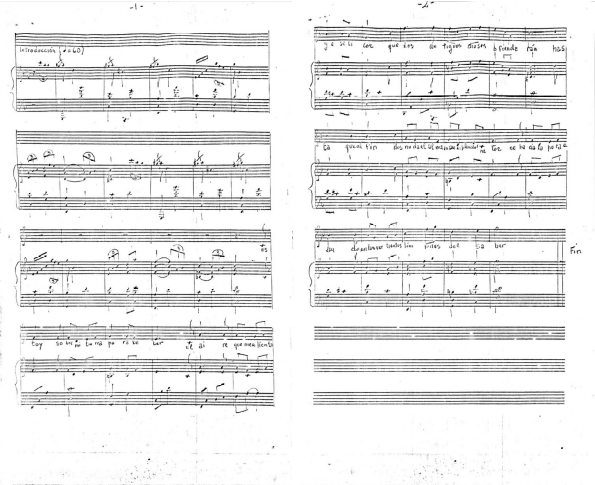
\includegraphics[width=1.0\textwidth]{img/partitura-original}
\caption{Copia del manuscrito del himno de Gustavo Leguizamón.}
\label{fig:partitura}
\end{figure}

\section{La caligrafía del manuscrito}
\label{sec:caligrafia}

\begin{figure}[H]
\begin{minipage}{\textwidth}
\centering
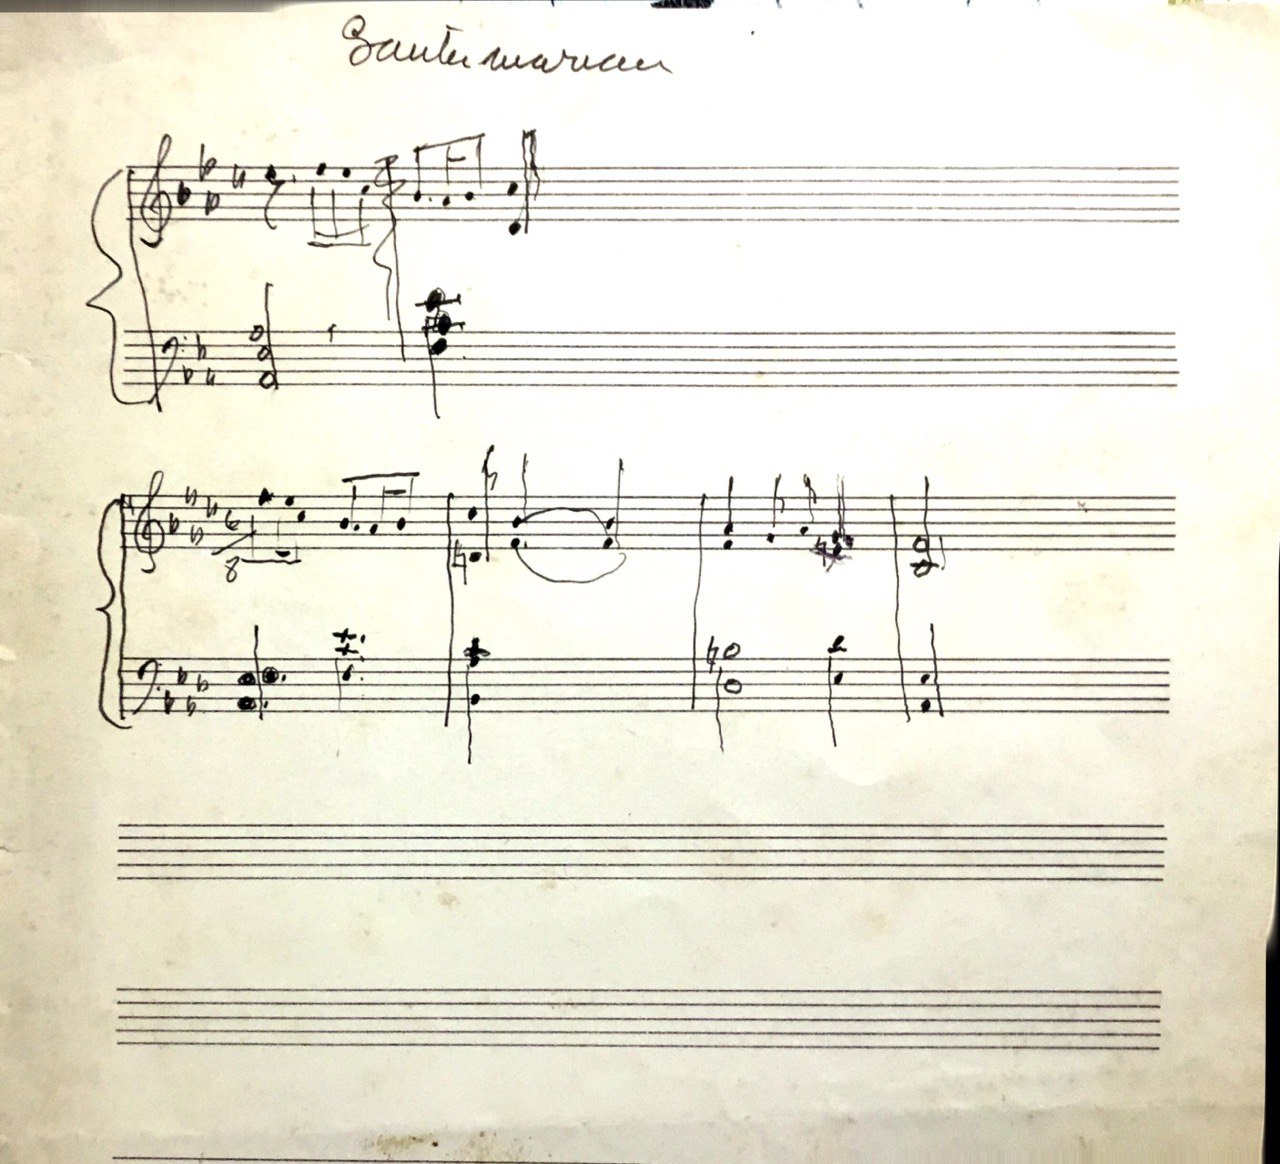
\includegraphics[width=0.6\textwidth]{img/manuscrito1}\\
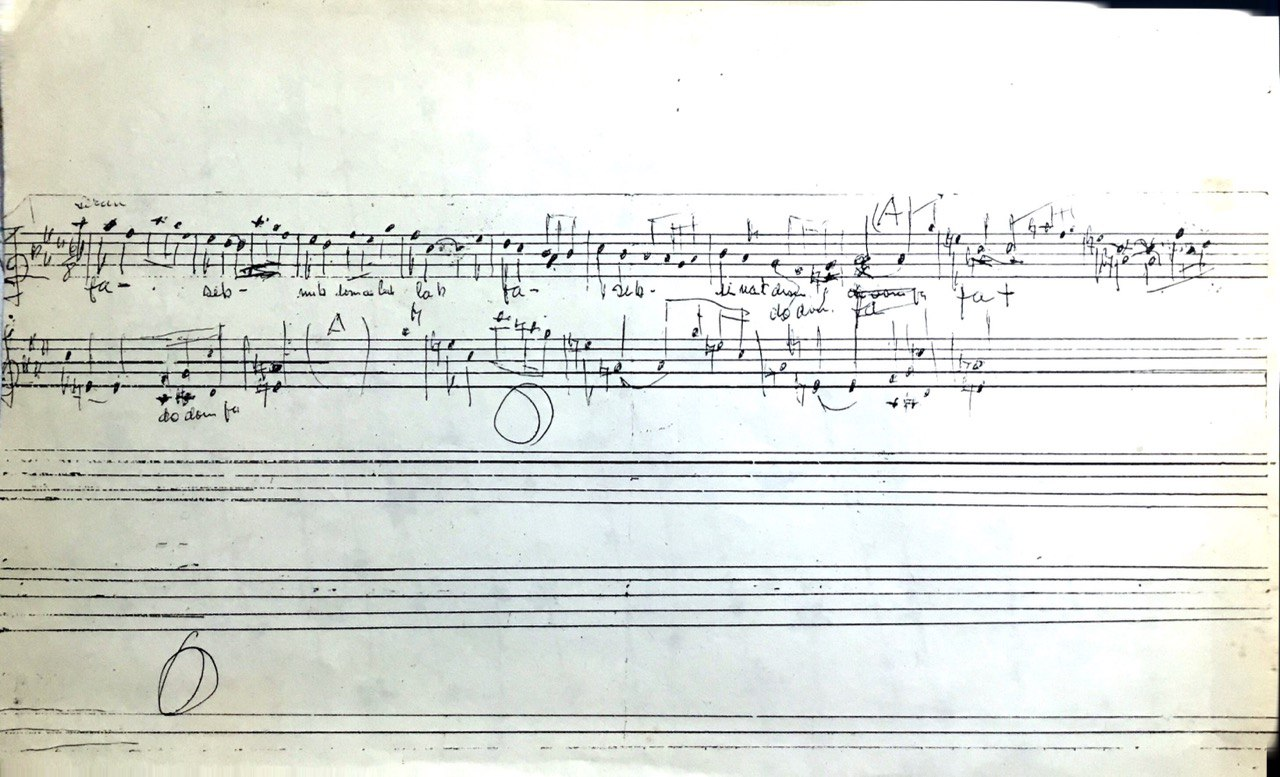
\includegraphics[width=0.6\textwidth]{img/manuscrito2}
\caption[Dos fragmentos de la caligrafía de Gustavo Leguizamón.]{Dos fragmentos\footnote{Fragmentos facilitados pon \textsc{Juan Martín Leguizamón}.} de la caligrafía de Gustavo Leguizamón.}
\label{fig:manuscritos}
\end{minipage}
\end{figure}

Si comparamos la caligrafía de la Figura~\ref{fig:partitura} (o el Apéndice de la página~\pageref{apx:partitura}, fotografía con mayor resolución) y la Figura~\ref{fig:manuscritos}, se hace evidente a simple vista que es la misma mano la que trazó todos esos signos. El testimonio de \textsc{Juan Martín Leguizamón} confirma que la letra sobre el primero de los fragmentos de la Figura~\ref{fig:manuscritos} es, efectivamente, la caligrafía de su padre.


\section{La grabación}
\label{sec:grabacion}

\begin{figure}[H]
\centering
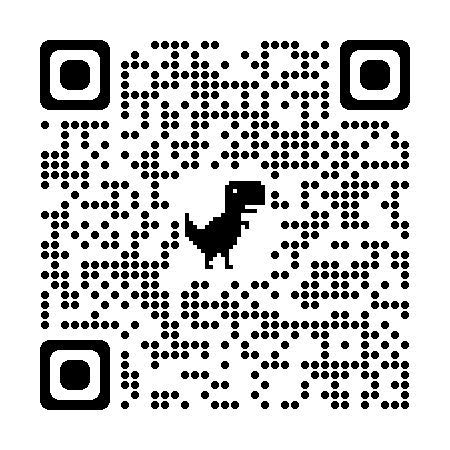
\includegraphics[width=0.3\textwidth]{img/qrcode-himno-fernandez}
\caption[La grabación del \emph{Himno}.]{La grabación del \emph{Himno a la Universidad Nacional de Salta}, en versión maquetada en el acompañamiento de piano y con la voz de \textsc{Federico Fernández}. URL: \url{https://drive.google.com/file/d/1KSCSEE7Ia5P0S9kFswWQibTyQr-1Ecdw/view?usp=drive_link}}
\label{fig:grabacion}
\end{figure}

Con el fin de acercar una versión sonora de la pieza presentada en concurso por Leguizamón y Pérez, \textsc{Federico Fernández}\footnote{\textsc{Federico Fernández} es destacadísimo músico y docente salteño, compositor, guitarrista, vocalista y contrabajista.} puso su voz y su conocimiento en manipulación de audio digital para esta versión que acá presentamos. Una advertencia: la pista de piano no está tocada por su ser humano, sino que es una simple maqueta de computadora basada en la versión MIDI generada por LilyPond. La falta de musicalidad de esta pista le resta calidad interpretativa a esta versión, aunque, a pesar de esta condición, se puede percibir el trabajo de Fernández sobre el fraseo de la melodía.


\section{Notas editoriales}
\label{sec:notas-editoriales}

La partitura manuscrita de Leguizamón (ver Figura~\ref{fig:partitura}) presenta algunos errores ortográficos que, a modo de corrección editorial, modificamos en la versión digitalizada de la página~\pageref{partitura-digitalizada}. A continuación, pormenorizamos y justificamos los cambios realizados.

En la línea intermedia en los primeros compases de la introducción hay un descenso cromático \hbox{\musncp{\key f \major d''2 cis'' c'' }.} El \hbox{\nota{do\sostenidotxt}{5},} en su significado musical. no es una nota descendente sino todo lo contrario; por eso corresponde escribir \hbox{\musncp{d''2 des'' c''}.}

En el compás 8, en la mano derecha encontramos un \musncp{dis'} en un acorde \acorde.V..\bemoltxt9.7.\sostenidotxt3./II, es decir \hbox{\musncp{<d' fis' a' c'' es''>}.} Por supuesto, ese \nota{mi\bemoltxt}{4} se dirige, en el pulso siguiente, a \nota{re}{4} \hbox{\musncp{<es' fis' c''>\glissando d' },} lo que justifica doblemente el cambio de \nota{re\sostenidotxt}{4} a \nota{mi\bemoltxt}{4}. El caso se repite de manera similar en el compás 16.

En los compases 33 y 34, una voz intermedia desciende cromáticamente \musncp{\clef alto \key f \major b bes a}. Al estar distribuida dicha voz entre las manos derecha (el \nota{si\becuadrotxt}{3}) e izquierda (el \nota{si\bemoltxt}{3} de compás 33 y el \nota{la}{3} de compás 34), se hace, aunque no necesario, preferible aclarar el \musncp[voffset=4pt]{\clef bass \key f \major bes?} con la alteración sobreentendida por armadura de clave con su notación de precaución, encerrada entre paréntesis.

En el penúltimo compás, el \nota{la\bemoltxt}{4} de la mano derecha se cambió por \nota{sol\sostenidotxt}{4} por ser éste la quinta aumentada del acorde de dominante de Fa mayor, el cual se dirige ascendiendo por semitono al \nota{la}{4} del acorde final.


\newpage
\section{Himno a la Universidad Nacional de Salta}\label{partitura-digitalizada}

\begin{flushright}
Música: \textsc{Gustavo Leguizamón}\\
Letra: \textsc{Miguel Ángel Pérez}
\end{flushright}

\lilypondfile[staffsize=11]{part/leguizamon-himno_unsa.ly}
